\section{Résultats des estimations}
\label{sec:resultats}

Cette section présente les résultats empiriques de la stratégie d'identification
PSM-Double différence. Elle s'organise en trois temps : l'estimation du score de
propension et la vérification de la qualité de l'appariement, la présentation des
estimateurs de double différence brute, et enfin les résultats de l'estimateur PSM-DD
de l'effet moyen du traitement sur les traités (ATT), avec une analyse des impacts
par dimension de la pauvreté.

\subsection{Estimation du score de propension}

\subsubsection{Résultats du modèle probit}

Le score de propension est estimé par un probit au \emph{niveau de l'enfant},
et non du ménage. Ce choix découle de l'unité d'analyse retenue tout au long
du mémoire : c'est la privation de l'enfant qui constitue la variable de
résultat, et deux enfants d'un même ménage n'ont ni le même sexe, ni le même
âge, ni donc les mêmes dimensions MODA applicables. Apparier des ménages
reviendrait à traiter comme identiques des enfants dont les besoins mesurés
diffèrent.

L'échantillon d'estimation est le panel d'enfants suivis entre les deux
vagues, appariés par l'identifiant préchargé décrit en
section~\ref{sec:methodo} (17\,786 enfants, dont 17\,769 utilisés par le
probit). Cette restriction n'est pas une commodité : c'est la seule
construction dans laquelle le poids d'appariement calculé à la période de base
se rapporte au \emph{même} individu à la seconde vague, condition d'une double
différence individuelle.

Les covariables combinent deux niveaux. Celles du ménage à la période de base
reprennent les déterminants des transferts retenus dans la littérature
\parencite{adams2005,gubert2002} : log de la dépense par tête, taille du
ménage, sexe, âge, niveau d'éducation et état matrimonial du chef, milieu et
région de résidence. S'y ajoutent celles de l'enfant : son sexe et son âge.
Toutes sont mesurées avant l'observation des résultats.

\begin{table}[H]
  \centering
  \caption{Modèle probit pour l'estimation du score de propension (EHCVM I, 2018-2019)}
  \label{tab:probit}
  \zebre
  \begin{tabular}{|l|c|c|}
    \hline
\entete Variable & Coefficient & Éc.-t. (cluster) \\
    \hline
    \textit{Caractéristiques de l'enfant} & & \\ \hline
    \quad Sexe féminin                         & $0{,}018$ & $(0{,}024)$ \\ \hline
    \quad Âge de l'enfant (années)             & $0{,}003$ & $(0{,}003)$ \\ \hline
    \textit{Caractéristiques du chef de ménage} & & \\ \hline
    \quad Âge du chef (années)                 & $0{,}005^{**}$ & $(0{,}003)$ \\ \hline
    \quad Chef féminin                         & $0{,}584^{***}$ & $(0{,}085)$ \\ \hline
    \quad Éducation : secondaire gén.~2        & -$0{,}420^{**}$ & $(0{,}195)$ \\ \hline
    \quad Divorcé(e)                           & -$1{,}082^{***}$ & $(0{,}385)$ \\ \hline
    \textit{Caractéristiques du ménage} & & \\ \hline
    \quad Taille du ménage                     & $0{,}048^{***}$ & $(0{,}006)$ \\ \hline
    \quad Log dépense par tête                 & $0{,}583^{***}$ & $(0{,}074)$ \\ \hline
    \quad Milieu rural                         & -$0{,}093$ & $(0{,}079)$ \\ \hline
    \textit{Effets fixes région}               & \multicolumn{2}{|c|}{Oui} \\
    \hline
    Constante                                  & -$9{,}95^{***}$ & $(1{,}031)$ \\
    \hline
    Pseudo-$R^2$ de McFadden                   & \multicolumn{2}{|c|}{$0{,}143$} \\ \hline
    Observations (enfants, panel suivi $t=0$)  & \multicolumn{2}{|c|}{$17\,769$} \\
    \hline
  \end{tabular}

  {\footnotesize \textit{Source :} Calcul de l'auteur, EHCVM. $^{*}p<0{,}10$, $^{**}p<0{,}05$, $^{***}p<0{,}01$~; écarts-types clusterisés par grappe entre parenthèses.}
\end{table}

Le modèle présente un pseudo-$R^2$ de McFadden de 14,3\,\%. Les déterminants
sont conformes à la littérature : la probabilité qu'un enfant vive dans un
ménage bénéficiaire croît fortement avec la dépense par tête ($0{,}58$), la
présence d'une femme à la tête du ménage ($0{,}58$), la taille du ménage
($0{,}05$) et l'âge du chef. Le coefficient de la dépense par tête signale une
sélection positive : ce sont les ménages les moins contraints qui ont pu
financer un départ à l'étranger. Celui du chef féminin reflète la
configuration migratoire typique où l'époux émigré laisse la gestion du ménage
à son épouse, configuration au c\oe{}ur du canal \og absence parentale \fg{}
discuté en section~\ref{sec:discussion}.

Les deux covariables individuelles ne sont en revanche pas significatives : ni
le sexe de l'enfant ($0{,}018$~; $p = 0{,}458$) ni son âge ($0{,}003$~;
$p = 0{,}355$) ne prédisent l'appartenance à un ménage bénéficiaire, ce qui
était attendu puisque le traitement est reçu au niveau du ménage. Leur
présence dans le modèle ne vise pas à améliorer la prédiction mais à garantir
que chaque enfant traité soit comparé à des enfants témoins de même sexe et de
même âge, donc évalués sur les mêmes dimensions MODA.

\subsubsection{Vérification de la qualité de l'appariement}

La figure~\ref{fig:support} représente les distributions du score de propension
des enfants bénéficiaires ($D=1$) et non bénéficiaires ($D=0$). Les deux
distributions se recouvrent sur l'essentiel de leur support ; les enfants
bénéficiaires situés dans la zone de support commun sont tous retenus et
appariés par la méthode des $k$ plus proches voisins (k-NN, $k=4$, avec
remise), pour un panel apparié de 15\,916 observations-enfants.

\begin{figure}[H]
  \centering
  \caption{Distribution du score de propension : enfants de ménages bénéficiaires et non bénéficiaires (EHCVM I, panel suivi)}
  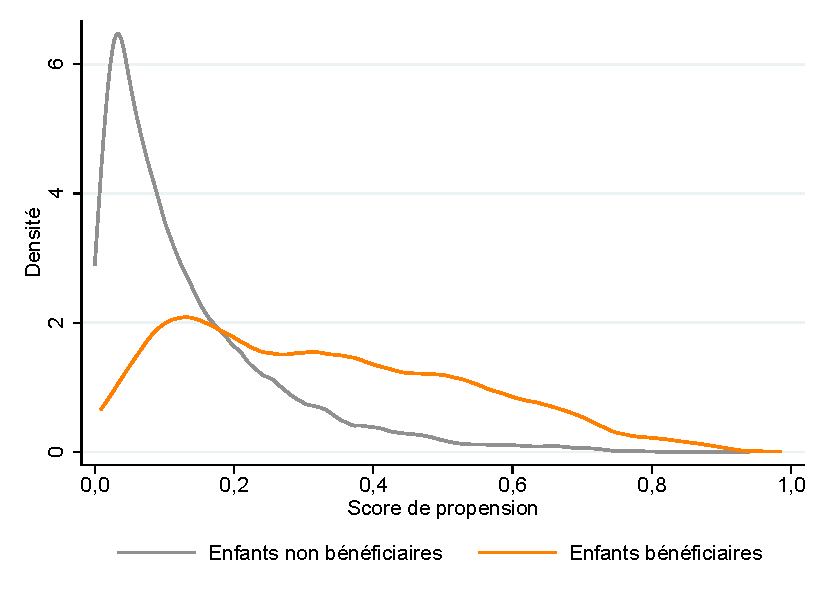
\includegraphics[width=0.85\linewidth]{figures/overlap_panel.pdf}
  \label{fig:support}

  {\footnotesize \textit{Source :} Calcul de l'auteur, EHCVM.}
\end{figure}

Avant appariement, les déséquilibres sont marqués : la différence standardisée
moyenne atteint 12,7\,\%, avec des écarts allant jusqu'à 38\,\% sur le sexe du
chef de ménage et 36\,\% sur la taille du ménage. Le
tableau~\ref{tab:balance} présente le diagnostic d'équilibrage obtenu une fois
l'appariement k-NN effectué : pour chaque covariable, la moyenne chez les
enfants bénéficiaires et chez leurs témoins appariés, la différence
standardisée et le test de Student associé. L'appariement corrige l'essentiel
des déséquilibres : la différence standardisée moyenne tombe à 2,9\,\%
(médiane 2,2\,\%), sous le seuil conventionnel de 10\,\%
\parencite{austin2009}, le pseudo-$R^2$ du probit réestimé sur l'échantillon
apparié passe de 0,143 à 0,006, et aucune différence résiduelle n'est
significative au seuil de 5\,\%. L'équilibrage porte aussi sur les covariables
individuelles, le sexe (SMD résiduelle de -$0{,}4$\,\%) et l'âge
(-$2{,}8$\,\%) de l'enfant.

\begin{table}[H]
  \centering
  \caption[Diagnostic post-appariement de l'équilibrage des covariables (méthode k-NN, niveau enfant)]{Diagnostic post-appariement de l'équilibrage des covariables (méthode k-NN, niveau enfant)\protect\footnotemark}
  \label{tab:balance}
  \zebre
  \small
  \resizebox{\linewidth}{!}{%
  \begin{tabular}{|l|c|c|c|c|c|}
    \hline
\entete Variable & Moyenne traités & Moyenne témoins & SMD (\%) & T-stat & $P>|t|$ \\
    \hline
    Sexe de l'enfant (\% filles) & 0,504 & 0,506 & -0,4 & -0,16 & 0,874 \\ \hline
    Âge de l'enfant (années)     & 6,873 & 6,992 & -2,8 & -1,00 & 0,317 \\ \hline
    Taille du ménage             & 12,45 & 12,25 & 2,7  & 0,46  & 0,644 \\ \hline
    Log dépense par tête         & 13,08 & 13,07 & 1,2  & 0,22  & 0,825 \\ \hline
    Milieu rural (\%)            & 0,391 & 0,392 & -0,2 & -0,04 & 0,970 \\
    \hline
  \end{tabular}%
  }

  {\footnotesize \textit{Source :} Calcul de l'auteur, EHCVM.}
\end{table}
\footnotetext{\textit{Note :} niveau enfant, panel de 17\,786 enfants suivis~; seuil conventionnel~: SMD $< 10\,\%$. Différence standardisée moyenne sur l'ensemble des covariables~: 12,7\,\% avant appariement, 2,9\,\% après.}

\subsection{Impact des transferts sur la pauvreté multidimensionnelle}

\subsubsection{Double différence sans appariement}

À titre de référence, nous estimons d'abord un estimateur de double
différence sans appariement (tableau~\ref{tab:dd_brut}). L'impact estimé est
de $+3{,}2$ points de pourcentage et non significatif ($p = 0{,}167$). Cette
comparaison brute reste toutefois exposée aux différences initiales entre les
deux groupes -- les bénéficiaires sont plus aisés, plus urbains, plus souvent
dirigés par une femme --, d'où le recours à l'appariement.

\begin{table}[H]
  \centering
  \caption[Estimations par double différence (DD brute, sans appariement)]{Estimations par double différence (DD brute, sans appariement)\protect\footnotemark}
  \label{tab:dd_brut}
  \zebre
  \begin{tabular}{|l|c|c|c|}
    \hline
\entete Variable de résultat & ATT$_{\text{DD}}$ & Éc.-t. (cluster) & $p$-valeur \\
    \hline
    Pauvreté MODA ($\hat{H}_{\text{MODA}}$) & $0{,}032$ & $(0{,}023)$ & 0,167 \\
    \hline
  \end{tabular}

  {\footnotesize \textit{Source :} Calcul de l'auteur, EHCVM.}
\end{table}
\footnotetext{\textit{Note :} erreurs-types clusterisées par grappe, $n = 53\,679$~; $\delta$ de $Y_{it} = \alpha + \beta t + \gamma D + \delta(t \times D) + \varepsilon_{it}$.}

\subsubsection{Estimateur par appariement et double différence}
\label{subsec:psmdd}

Le tableau~\ref{tab:psmdd_att} rapporte les estimations de l'ATT par l'estimateur
PSM-DD de \textcite{heckman1997,heckman1998}, qui combine l'appariement par score
de propension et la double différence pour éliminer simultanément les biais de
sélection sur observables et les effets fixes inobservables constants dans le temps.

\begin{table}[H]
  \centering
  \caption[Impact des transferts sur la pauvreté multidimensionnelle : estimateur PSM-DD (ATT)]{Impact des transferts sur la pauvreté multidimensionnelle : estimateur PSM-DD (ATT)\protect\footnotemark}
  \label{tab:psmdd_att}
  \zebre
  \begin{tabular}{|l|c|c|c|}
    \hline
\entete Variable de résultat & ATT & Éc.-t. (cluster) & $p$-valeur \\
    \hline
    \multicolumn{4}{|c|}{\textit{Approche MODA (7 dimensions, $k=4$)}} \\ \hline
    \quad Incidence $\hat{H}_{\text{MODA}}$         & $0{,}053^{*}$ & $(0{,}031)$ & 0,086 \\
    \hline
  \end{tabular}

  {\footnotesize \textit{Source :} Calcul de l'auteur, EHCVM. $^{*}p<0{,}10$.}
\end{table}
\footnotetext{\textit{Note :} appariement k-NN au niveau enfant, erreurs-types clusterisées par grappe, $n = 15\,916$ observations-enfants.}

L'estimateur PSM-DD donne un ATT de $0{,}053$, significatif au seuil de
10\,\% mais non au seuil de 5\,\% ($p = 0{,}086$). Le signe est positif :
entre 2018-2019 et 2021-2022, la privation multidimensionnelle des enfants de
ménages bénéficiaires a reculé \emph{plus lentement} que celle d'enfants
témoins de sexe, d'âge et de profil de ménage comparables, l'écart étant de
l'ordre de 5 points de pourcentage.

Deux conclusions s'imposent. D'abord, l'hypothèse H1 n'est pas validée : les
transferts ne réduisent pas la pauvreté multidimensionnelle des enfants sur
l'horizon observé. Ensuite, la lecture inverse -- celle d'un effet défavorable
-- ne peut être affirmée avec la fermeté qu'exige une conclusion causale :
l'intervalle de confiance à 95\,\% ($[-0{,}8~;~11{,}4]$ points) contient zéro,
et la significativité au seuil de 10\,\% relève d'une présomption plutôt que
d'une démonstration. Cette présomption est toutefois cohérente sur l'ensemble
des spécifications, et la section~\ref{sec:discussion} en examine les canaux
possibles.

La figure~\ref{fig:dd_trajectoires} illustre le mécanisme de la double
différence. Elle représente l'incidence MODA des enfants bénéficiaires et des
témoins appariés aux deux vagues, ainsi que le contrefactuel obtenu en
appliquant la tendance des témoins au niveau initial des bénéficiaires ;
l'écart entre la trajectoire observée des bénéficiaires et son contrefactuel
correspond à l'ATT estimé.

\begin{figure}[H]
  \centering
  \caption{Illustration de la double différence : trajectoires des bénéficiaires,
 	des témoins appariés et contrefactuel (incidence MODA)}
  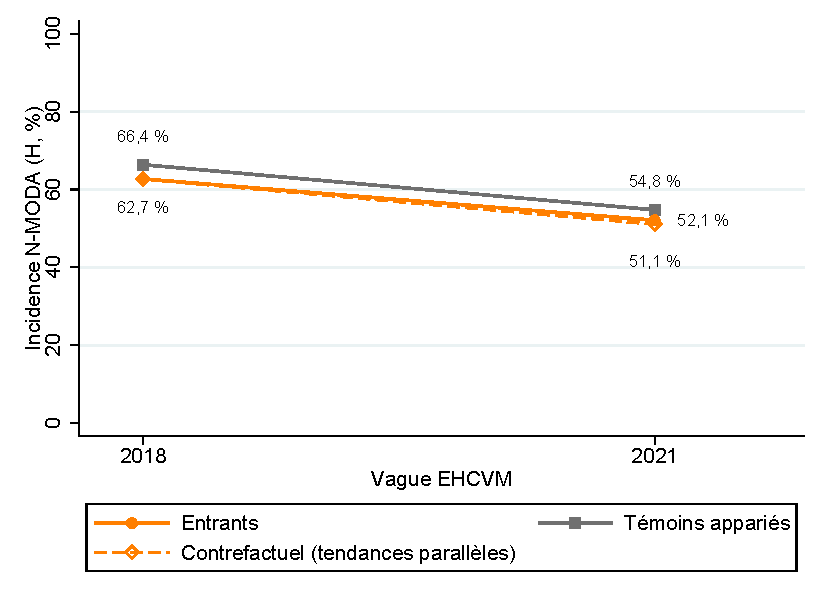
\includegraphics[width=0.85\linewidth]{figures/fig_dd_trajectoires.pdf}
  \label{fig:dd_trajectoires}

  {\footnotesize \textit{Source :} Calcul de l'auteur, EHCVM.}
\end{figure}

\subsubsection{Robustesse au choix de la méthode d'appariement}

Le tableau~\ref{tab:psm_methodes} examine la stabilité des résultats selon la
méthode d'appariement retenue. Les trois algorithmes concordent étroitement :
l'ATT vaut $0{,}053$ pour le k-NN ($p = 0{,}086$), $0{,}060$ pour le noyau
Epanechnikov ($p = 0{,}074$) et $0{,}050$ pour le caliper ($p = 0{,}057$),
tous trois significatifs au seuil de 10\,\% et aucun au seuil de 5\,\%. La
double différence brute, qui ne corrige pas la sélection, donne une valeur
plus faible et non significative ($0{,}032$~; $p = 0{,}167$) : c'est
l'appariement qui fait apparaître l'écart de trajectoire, en neutralisant
l'avantage initial des enfants de ménages bénéficiaires.

\begin{table}[H]
  \centering
  \caption[Sensibilité de l'ATT PSM-DD au choix de la méthode d'appariement]{Sensibilité de l'ATT PSM-DD au choix de la méthode d'appariement\protect\footnotemark}
  \label{tab:psm_methodes}
  \zebre
  \begin{tabular}{|l|c|c|}
    \hline
\entete Méthode d'appariement & ATT (MODA) & $p$-val. \\
    \hline
    k-NN ($k=4$, avec remise)             & $0{,}053^{*}$ & 0,086 \\ \hline
    Noyau Epanechnikov ($h=0{,}06$)       & $0{,}060^{*}$ & 0,074 \\ \hline
    Caliper ($\varepsilon = 0{,}05$, sans remise) & $0{,}050^{*}$ & 0,057 \\ \hline
    DD brute (sans appariement)           & $0{,}032$  & 0,167 \\
    \hline
  \end{tabular}

  {\footnotesize \textit{Source :} Calcul de l'auteur, EHCVM. $^{*}p<0{,}10$.}
\end{table}
\footnotetext{\textit{Note :} erreurs-types clusterisées par grappe, appariement au niveau enfant.}

\subsubsection{Sensibilité au seuil de privation \texorpdfstring{$k$}{k}}
\label{subsec:sensib_k}

Le seuil $k=4$ dimensions sur sept retenu pour déclarer un enfant pauvre est
une convention. Le tableau~\ref{tab:sensib_k} réestime l'ATT en le faisant
varier de $k=3$ à $k=6$, ce qui fait passer l'incidence de 75,1\,\% à
13,3\,\% sur le panel apparié à la période de base. Le signe de l'effet est
positif à chaque seuil et son ampleur décroît avec la sévérité : $5{,}2$ pp à
$k=3$, $5{,}3$ pp à $k=4$, $3{,}4$ pp à $k=5$ et $2{,}9$ pp à $k=6$. La
significativité suit la même pente : l'effet est significatif à 5\,\% pour la
définition la plus inclusive ($p = 0{,}042$), à 10\,\% au seuil de référence
($p = 0{,}086$), et ne l'est plus au-delà.

Cette structure a un sens économique. Les transferts pèsent sur la marge, là
où quelques privations font basculer un enfant de part et d'autre du seuil, et
non sur le noyau des enfants cumulant six ou sept privations, dont la
situation relève de déficits structurels qu'un flux monétaire ne déplace pas.
La conclusion d'ensemble ne dépend donc pas du choix conventionnel de $k=4$ ;
c'est son intensité qui varie.

\begin{table}[H]
  \centering
  \caption[Sensibilité de l'ATT PSM-DD au seuil inter-dimensionnel $k$]{Sensibilité de l'ATT PSM-DD au seuil inter-dimensionnel $k$\protect\footnotemark}
  \label{tab:sensib_k}
  \zebre
  \begin{tabular}{|c|c|c|c|c|}
    \hline
\entete Seuil $k$ & Incidence 2018 (\%) & ATT & Éc.-t. (cluster) & $p$-valeur \\
    \hline
    3 & 75,1 & $0{,}052^{**}$ & $(0{,}026)$ & 0,042 \\ \hline
    4 & 54,4 & $0{,}053^{*}$  & $(0{,}031)$ & 0,086 \\ \hline
    5 & 31,8 & $0{,}034$      & $(0{,}027)$ & 0,205 \\ \hline
    6 & 13,3 & $0{,}029$      & $(0{,}021)$ & 0,175 \\
    \hline
  \end{tabular}

  {\footnotesize \textit{Source :} Calcul de l'auteur, EHCVM. $^{*}p<0{,}10$, $^{**}p<0{,}05$.}
\end{table}
\footnotetext{\textit{Note :} appariement k-NN au niveau enfant, erreurs-types clusterisées par grappe~; l'incidence est pondérée par \texttt{hhweight} sur le panel apparié à $t=0$.}

\subsubsection{Effets par dimension}

\begin{figure}[H]
  \centering
  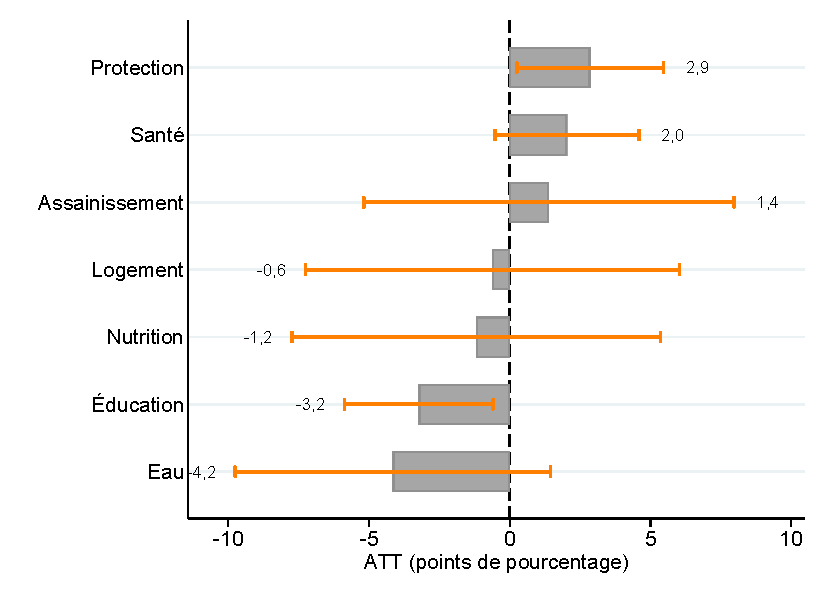
\includegraphics[width=0.85\linewidth]{figures/fig_effets_dim.pdf}
  \caption{Impact des transferts de migrants par dimension MODA (ATT PSM-DD, IC 95\,\%)}
  \label{fig:effets_dim}

  {\footnotesize \textit{Source :} Calcul de l'auteur, EHCVM.}
\end{figure}

L'analyse par dimension (figure~\ref{fig:effets_dim} et
tableau~\ref{tab:effets_dim}) décompose l'ATT global sur les sept dimensions
MODA. Une seule ressort : la \textbf{nutrition}, avec un ATT de $0{,}084$
significatif au seuil de 5\,\% ($p = 0{,}043$). La privation alimentaire des
enfants de ménages bénéficiaires recule 8,4 points plus lentement que celle de
leurs témoins appariés. C'est aussi la dimension la plus directement sensible
au budget courant du ménage, donc celle où un apport monétaire aurait dû se
voir en premier : le résultat va à l'encontre de l'effet attendu.

L'assainissement suit avec $0{,}069$, sans atteindre la significativité
($p = 0{,}109$). Les cinq autres dimensions présentent des coefficients
faibles et non significatifs ; l'éducation est rigoureusement nulle
($-0{,}0001$~; $p = 0{,}995$), et la protection de l'enfant, malgré son
contenu directement lié à l'absence parentale, ne se distingue pas
($0{,}019$~; $p = 0{,}345$).

Le volet dimensionnel de l'hypothèse H2 est donc partiellement validé :
l'effet des transferts n'est pas uniforme entre dimensions, il se concentre
sur la nutrition. Les deux autres volets de H2, relatifs au milieu de
résidence et au sexe de l'enfant, sont examinés en
section~\ref{sec:discussion}.

\begin{table}[H]
  \centering
  \caption[Impact des transferts par dimension MODA (ATT PSM-DD)]{Impact des transferts par dimension MODA (ATT PSM-DD)\protect\footnotemark}
  \label{tab:effets_dim}
  \zebre
  \begin{tabular}{|l|c|c|c|}
    \hline
\entete Dimension & ATT & Éc.-t. (cluster) & $p$-valeur \\
    \hline
    Nutrition            & $0{,}084^{**}$ & $(0{,}042)$ & 0,043 \\ \hline
    Assainissement       & $0{,}069$      & $(0{,}043)$ & 0,109 \\ \hline
    Logement             & $0{,}041$      & $(0{,}041)$ & 0,316 \\ \hline
    Protection           & $0{,}019$      & $(0{,}020)$ & 0,345 \\ \hline
    Santé                & $0{,}010$      & $(0{,}012)$ & 0,400 \\ \hline
    Eau                  & $0{,}003$      & $(0{,}029)$ & 0,928 \\ \hline
    Éducation            & -$0{,}000$     & $(0{,}016)$ & 0,995 \\
    \hline
  \end{tabular}

  {\footnotesize \textit{Source :} Calcul de l'auteur, EHCVM. $^{**}p<0{,}05$.}
\end{table}
\footnotetext{\textit{Note :} appariement k-NN au niveau enfant, erreurs-types clusterisées par grappe.}
